% --------------------------------------------------------------
% This is all preamble stuff that you don't have to worry about.
% Head down to where it says "Start here"
% --------------------------------------------------------------
 
\documentclass[12pt]{article}
\usepackage{graphicx}
\graphicspath{ {images/} }
 
\usepackage[margin=1in]{geometry} 
\usepackage{amsmath,amsthm,amssymb}
\setlength{\parskip}{1em}

\newcommand{\N}{\mathbb{N}}
\newcommand{\Z}{\mathbb{Z}}
 
\newenvironment{theorem}[2][Theorem]{\begin{trivlist}
\item [\hskip \labelsep {\bfseries #1}\hskip \labelsep {\bfseries #2.}]}{\end{trivlist}}
\newenvironment{lemma}[2][Lemma]{\begin{trivlist}
\item [\hskip \labelsep {\bfseries #1}\hskip \labelsep {\bfseries #2.}]}{\end{trivlist}}
\newenvironment{exercise}[2][Exercise]{\begin{trivlist}
\item [\hskip \labelsep {\bfseries #1}\hskip \labelsep {\bfseries #2.}]}{\end{trivlist}}
\newenvironment{problem}[2][Problem]{\begin{trivlist}
\item [\hskip \labelsep {\bfseries #1}\hskip \labelsep {\bfseries #2.}]}{\end{trivlist}}
\newenvironment{question}[2][Question]{\begin{trivlist}
\item [\hskip \labelsep {\bfseries #1}\hskip \labelsep {\bfseries #2.}]}{\end{trivlist}}
\newenvironment{corollary}[2][Corollary]{\begin{trivlist}
\item [\hskip \labelsep {\bfseries #1}\hskip \labelsep {\bfseries #2.}]}{\end{trivlist}}

\newenvironment{solution}{\begin{proof}[Solution]}{\end{proof}}
 
\begin{document}
 
% --------------------------------------------------------------
%                         Start here
% --------------------------------------------------------------
 
\title{Week 3 Writeup}
\author{Arthur Liou}

\maketitle

Prompt: Submitting a write-up of your thoughts, impressions, and any conclusions based on the material from the week. Each week will have its own assignment in the grades page.
\par
\linebreak
	For this week’s writeup, I’m reflecting on the lectures content that we had over the two lessons (and multiple videos per lesson). This week, we went over Malware Defense and went through the YARA and Cuckoo labs. We also reviewed an attach graph in the first lesson that illustrate the typical breakdown of the procedural steps malware takes when it attacks. I found the idea of these steps to be straightforward and it made sense / nothing really surprised me. While informative, the YARA Lab pales in comparison to the Cuckoo lab, due to the process of automation and scale, which was covered in the beginning part of the second lesson. I also found the visuals of the procedures very useful, and I added those in my notes below.

\newpage
Lecture Notes
\newline
Malware Defenses Lesson 1
\begin{itemize}
\item	Goal this week: Gain an understanding and experience in the role of a malware researcher, primarily from Windows host-based protection.
\item	This is an attack graph that represents the vast majority of malware attacks on a user/system.  We’re going to break down the sections such that by the end of the class, you’ll have a good mid-to-high level of understanding.
o	Execute code on the system
o	Blend in or Hide
o	Persist
o	Harvest information
o	Phone home
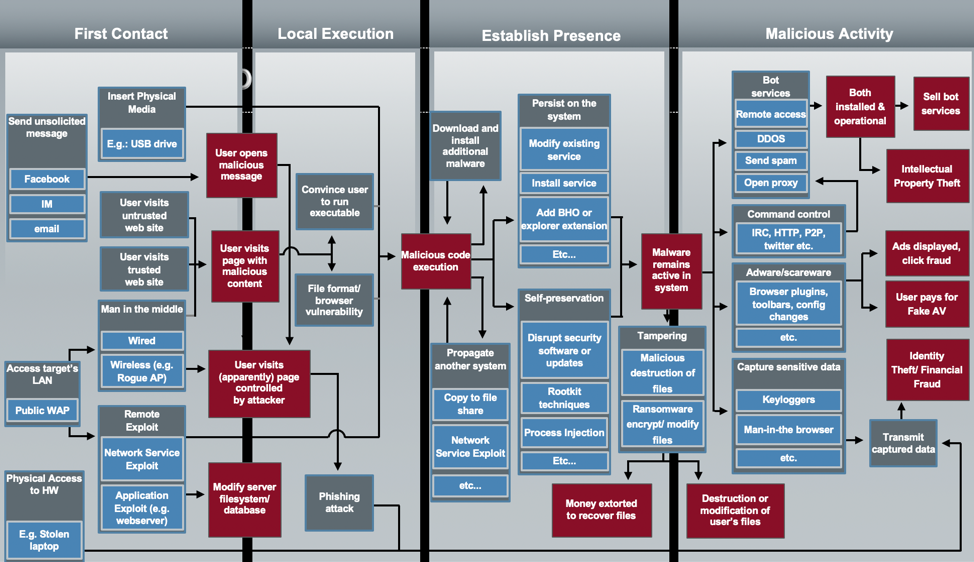
\includegraphics{Picture1.png}

\item	Add some channels here: email, IM, compromised sites and servers, malvertising, physical access (USB), etc
o	Social engineering: Social networks, IM, Email, 
o	Exploitation: Watering hole attacks, malvertising, physical access
o	Combination: Poisoned search results, 
o	Physical access:
o	Social engineering: Users knowingly run executable (copy cat apps)
o	Exploitation: Browser-based exploit kits (script, pdf, java)
o	Abusing features: USB Autorun, physical access,
\item	Establish presence Slide – Persist – System Startup, Windows Startup, Application Startup, Other such as scheduled tasks.
\item	Proxy Auto Config http://securelist.com/blog/virus-watch/29680/benign-feature-malicious-use/
\item	Run Keys - https://www.virusbtn.com/virusbulletin/archive/2014/03/vb201403-Simbot#id3507994
\item	Local Execution – Harvest information – enumerate (pw, docs, emails, processes)
\item	Hook (browser, keylog, screenscrap), Parse (pw, CC), Logs, Phone home, web, email
\item	First Contact
o	Spam: Anti-spam
o	Network: Firewall, Network IPS
o	Web: IP, Domain, & URL reputation
o	Physical access: Disk encryption
\item	Local Execution
o	Spam: Client-side content filtering
o	Network: Network IPS
o	Web: Content filtering/scanning
o	Host: Host IPS, Anti-virus, Whitelisting
\item	Establish Presence
o	Host: Anti-virus, Whitelisting, HIPS
o	Network: Firewall, Network IPS
o	Web: IP, Domain, & URL reputation
\item	Malicious Activity
o	Host: Anti-virus
o	Network: NIPS, Firewall
o	Web: IP, Domain, URL rep & content filtering
o	Data Loss Prevention
\item	Malware Def – Popular Tech – Network Firewall, Network Intrusion Prevention, Message Reputation, Network Reputation, Web Reputation, Host Firewall, Host IPS, Access Control, Anti-malware
\item	Content Engines interpret Content Rules, that define what is good or bad
\item	EndPoint Dependencies – Management Server, Point Product, Scanner Core, Engine, Content
\item	Anti-malware features: Traditional File Scanning (OAS, ODS), Registry & Cookies, Cloud scanning, Memory Scanning, Scripts, Heuristics, Decomposition, Configuration: Exclusions, Sensitivity, Reporting, etc
\item	YARA - The pattern matching Swiss knife for malware researchers
o	String expression, byte patterns, 
\item	LAB / Code.google YARA Broswer - Using Yara to Author Static File Signatures (I have a lot more notes / code below, but did not add them to my Latex, they're in my supplemental file)

\end{itemize}

\newline
Malware Defenses Lesson 2
\begin{itemize}
\item	Over half-a-million new and unique malicious binaries discovered each day
\item	Deep analysis is not possible for the vast majority of threats, need automation.
\item	Advantages of anti-malware automation?
o	Scale
o	Consistency
o	Performance less of a concern (paranoid heuristics)
\item	Disadvantages?
o	Out of context
o	Prone to evasion
o	Potentially prone to probing and DoS attacks
\item	cuckoo automated analysis
o	Source: http://docs.cuckoosandbox.org/en/latest/introduction/what/
o	Cuckoo is an automated malware analysis system: a tool that allows you to understand what a given file does when executed inside an isolated environment.
o	Bypass sleep bombs by intelligently skipping sleeps
o	Emulate user interaction by moving mouse and pushing buttons
o	Randomizes the system clock with each run
o	Uses a randomly named cuckoomon.dll

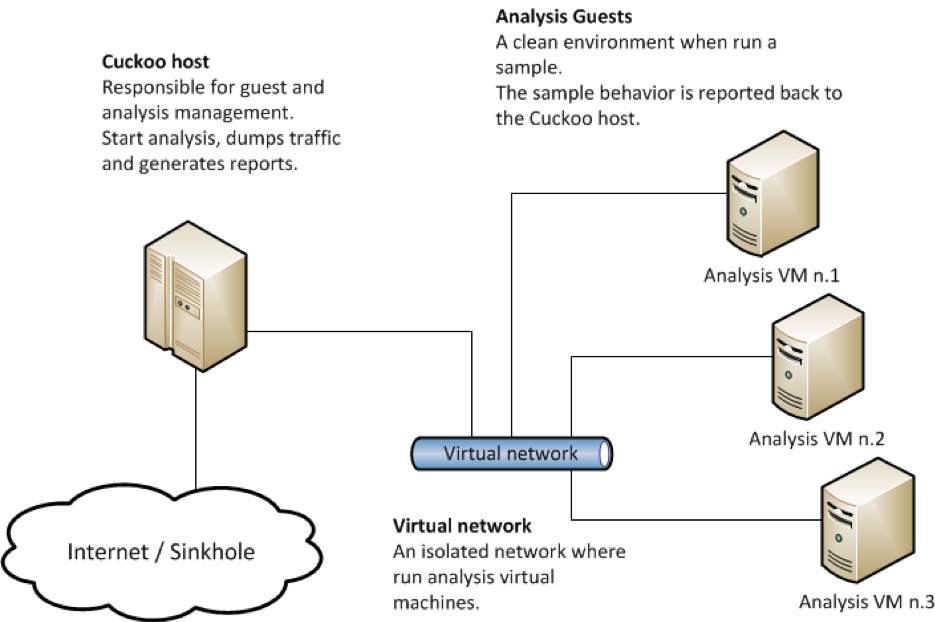
\includegraphics{Picture2.png}

\item	Cuckoo Design
\item	Source: http://docs.cuckoosandbox.org/en/latest/introduction/what/
\item	Cuckoo Replication in VM
\item	Malware Analysis aims to:
o	Discover if a threat is present
o	Isolate, Classify, and Remediate the malicious code
o	Defend against future attacks
o	Describe the attack
\item	Lab – Putting It All Together - altogether

\end{itemize}

% --------------------------------------------------------------
%     You don't have to mess with anything below this line.
% --------------------------------------------------------------
 
\end{document}
